\documentclass[aspectratio=169]{../latex_main/tntbeamer}  % you can pass all options of the beamer class, e.g., 'handout' or 'aspectratio=43'
\usepackage{dsfont}
\usepackage{bm}
\usepackage[english]{babel}
\usepackage[T1]{fontenc}
%\usepackage[utf8]{inputenc}
\usepackage{graphicx}
\graphicspath{ {./figures/} }
\usepackage{algorithm}
\usepackage[ruled,vlined,algo2e,linesnumbered]{algorithm2e}
\usepackage{hyperref}
\usepackage{booktabs}
\usepackage{mathtools}

\usepackage{amsmath,amssymb}

\DeclareMathOperator*{\argmax}{arg\,max}
\DeclareMathOperator*{\argmin}{arg\,min}

\usepackage{amsbsy}
\newcommand{\vect}[1]{\bm{#1}}
%\newcommand{\vect}[1]{\boldsymbol{#1}}

\usepackage{pgfplots}
\pgfplotsset{compat=1.16}
\usepackage{tikz}
\usetikzlibrary{trees} 
\usetikzlibrary{shapes.geometric}
\usetikzlibrary{positioning,shapes,shadows,arrows,calc,mindmap}
\usetikzlibrary{positioning,fadings,through}
\usetikzlibrary{decorations.pathreplacing}
\usetikzlibrary{intersections}
\pgfdeclarelayer{background}
\pgfdeclarelayer{foreground}
\pgfsetlayers{background,main,foreground}
\tikzstyle{activity}=[rectangle, draw=black, rounded corners, text centered, text width=8em]
\tikzstyle{data}=[rectangle, draw=black, text centered, text width=8em]
\tikzstyle{myarrow}=[->, thick, draw=black]

% Define the layers to draw the diagram
\pgfdeclarelayer{background}
\pgfdeclarelayer{foreground}
\pgfsetlayers{background,main,foreground}

% Requires XeLaTeX or LuaLaTeX
%\usepackage{unicode-math}

\usepackage{fontspec}
%\setsansfont{Arial}
\setsansfont{RotisSansSerifStd}[ 
Path=../latex_main/fonts/,
Extension = .otf,
UprightFont = *-Regular,  % or *-Light
BoldFont = *-ExtraBold,  % or *-Bold
ItalicFont = *-Italic
]
\setmonofont{Cascadia Mono}[
Scale=0.8
]

% scale factor adapted; mathrm font added (Benjamin Spitschan @TNT, 2021-06-01)
%\setmathfont[Scale=1.05]{Libertinus Math}
%\setmathrm[Scale=1.05]{Libertinus Math}

% other available math fonts are (not exhaustive)
% Latin Modern Math
% XITS Math
% Libertinus Math
% Asana Math
% Fira Math
% TeX Gyre Pagella Math
% TeX Gyre Bonum Math
% TeX Gyre Schola Math
% TeX Gyre Termes Math

% Literature References
\newcommand{\lit}[2]{\href{#2}{\footnotesize\color{black!60}[#1]}}

%%% Beamer Customization
%----------------------------------------------------------------------
% (Don't) Show sections in frame header. Options: 'sections', 'sections light', empty
\setbeamertemplate{headline}{empty}

% Add header logo for normal frames
\setheaderimage{
	% 
\includegraphics[height=\logoheight]{figures/TNT_darkv4.pdf}
	
\includegraphics[height=\logoheight]{../latex_main/figures/luh_logo_rgb_0_80_155.pdf}
	% 
\includegraphics[height=\logoheight]{figures/logo_tntluh.pdf}
}

% Header logo for title page
\settitleheaderimage{
	% 
\includegraphics[height=\logoheight]{figures/TNT_darkv4.pdf}
	
\includegraphics[height=\logoheight]{../latex_main/figures/luh_logo_rgb_0_80_155.pdf}
	% 
\includegraphics[height=\logoheight]{figures/logo_tntluh.pdf}
}

% Title page: tntdefault 
\setbeamertemplate{title page}[tntdefault]  % or luhstyle
% Add optional title image here
%\addtitlepageimagedefault{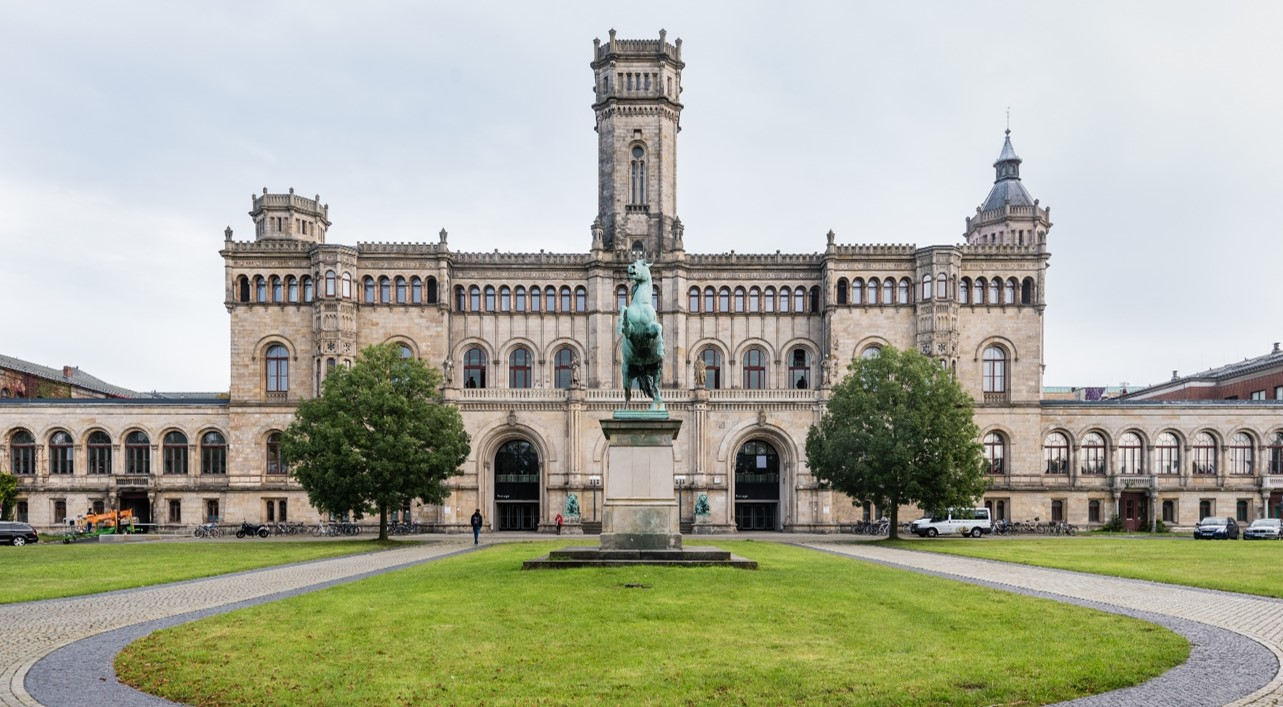
\includegraphics[width=0.65\textwidth]{figures/luh_default_presentation_title_image.jpg}}

% Title page: luhstyle
% \setbeamertemplate{title page}[luhstyle]
% % Add optional title image here
% \addtitlepageimage{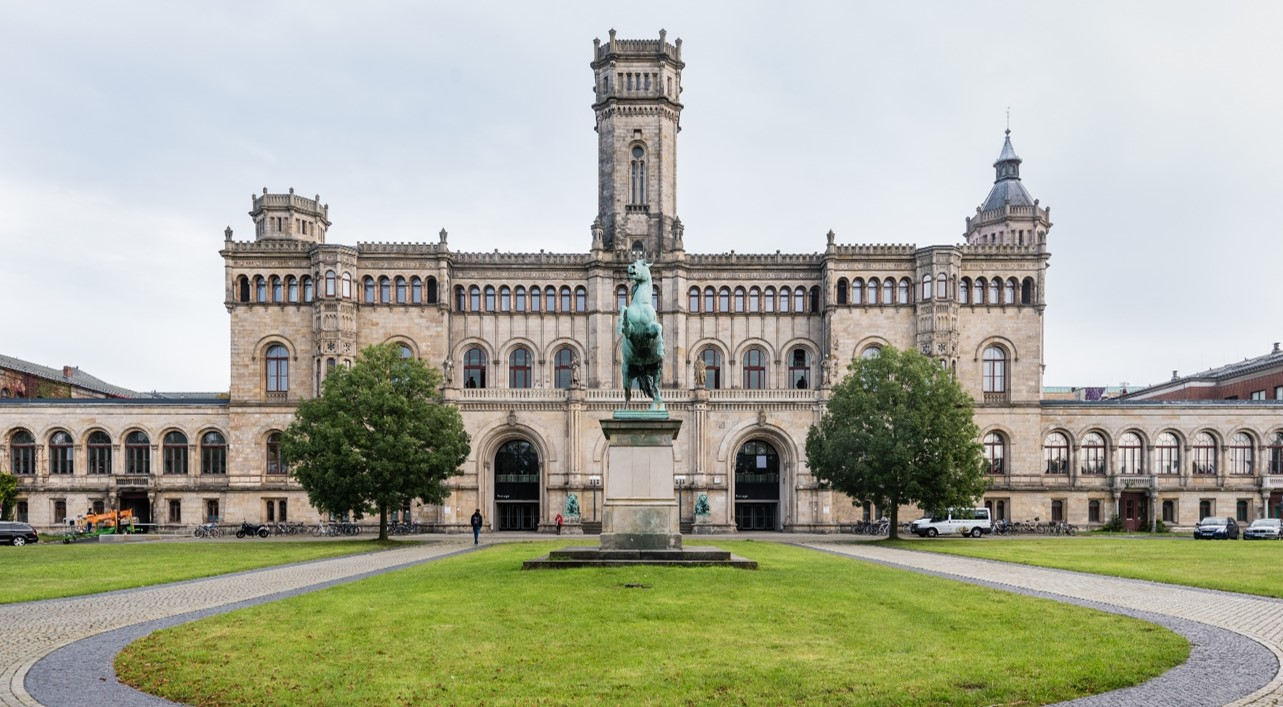
\includegraphics[width=0.75\textwidth]{figures/luh_default_presentation_title_image.jpg}}

\author[Abedjan \& Lindauer]{Ziawasch Abedjan \& Marius Lindauer\\[1em]
	
\includegraphics[height=\logoheight]{../latex_main/figures/luh_logo_rgb_0_80_155.pdf}\qquad
	
\includegraphics[height=\logoheight]{../latex_main/figures/DBIS_Kurzlogo.png}\qquad

\includegraphics[height=\logoheight]{../latex_main/figures/TNT_darkv4}\qquad

\includegraphics[height=\logoheight]{../latex_main/figures/L3S.jpg}	}
\date{Summer Term 2022; \hspace{0.5em} {
\includegraphics[height=1.5em]{../latex_main/figures/Cc-by-nc-sa_icon.svg.png}}; based on \href{https://ds100.org/fa21/}{[DS100]}
}


%%% Custom Packages
%----------------------------------------------------------------------
% Create dummy content
\usepackage{blindtext}

% Adds a frame with the current page layout. Just call \layout inside of a frame.
\usepackage{layout}


%%% Macros
%\renewcommand{\vec}[1]{\mathbf{#1}}
% \usepackage{bm}
%\let\vecb\bm

\title[Introduction]{DS: Estimation and Bias}
\subtitle{Random Variables}

\graphicspath{ {./figure/} }
%\institute{}


\begin{document}
	
	\maketitle
	\begin{frame}{Distributions and Data Generation}
	    \begin{columns}
	        \begin{column}{.3\textwidth}
	        Zoom Poll Data\\
	           \begin{figure}
	               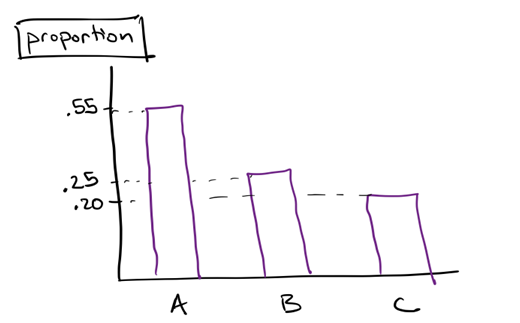
\includegraphics[scale=.5]{Bild10}
	           \end{figure}
	           Empirical Distribution: the distribution of your sample (values and proportions)
	        \end{column}
	        
	        \begin{column}{.3\textwidth}
	            Polling a student from full class
                \begin{figure}
                    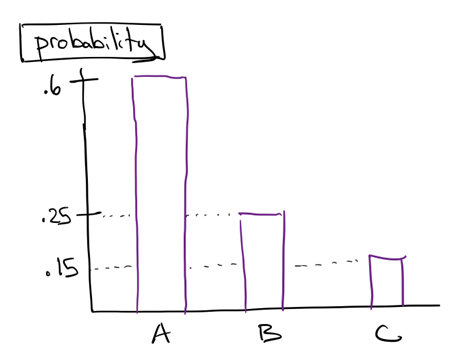
\includegraphics[scale=.5]{Bild11}
                \end{figure}
                Probability Distribution: a model for how the sample is generated (values and probabilities).
	        \end{column}
	        
	        
	        \begin{column}{.3\textwidth}
	            Note: Probability Distributions
	            \begin{itemize}
	                \item Can describe sampling from a population, but that’s not all
	                \begin{itemize}
	                    \item \# of pips on die roll
	                \end{itemize}
	                \item Often not known
	            \end{itemize}
                \begin{figure}
                    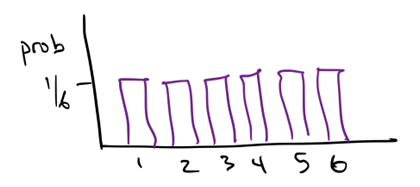
\includegraphics[scale=.5]{Bild12}
                \end{figure}
	        \end{column}
	    \end{columns}
	    
	\end{frame}
	
	
		\begin{frame}{Generating Data for FDR vs. Landon}
	    \begin{columns}
	        \begin{column}{.4\textwidth}
	       
	           \begin{figure}
	               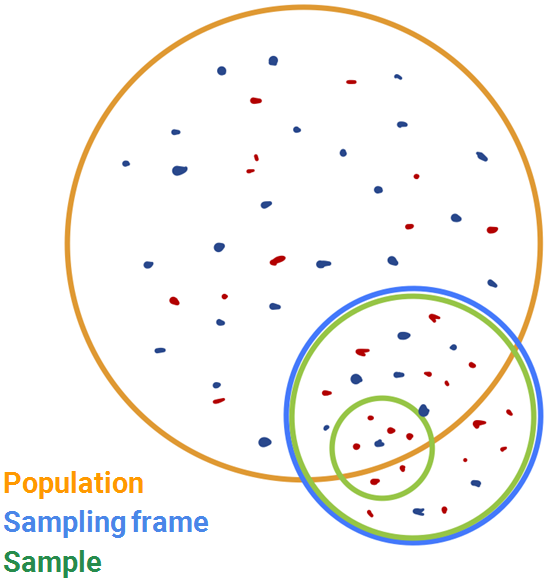
\includegraphics[scale=.37]{Bild13}
	           \end{figure}
	        \end{column}
	        
	        \begin{column}{.4\textwidth}
	           Probability Distributions\\
	           Sampling process 1: draw n = 10 million

	           
                \begin{figure}
                    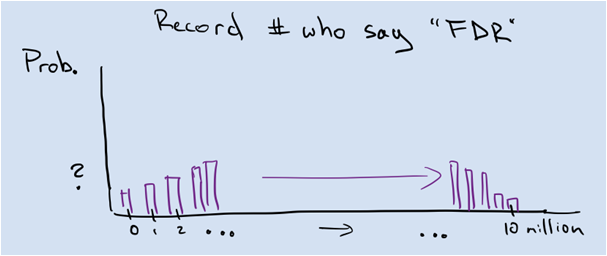
\includegraphics[scale=.4]{Bild14}
                \end{figure}
                Sampling process 2: draw n = 1 person
                \begin{figure}
                    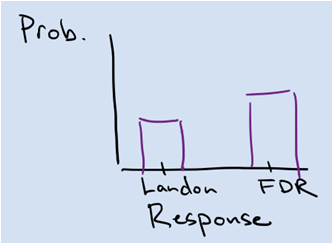
\includegraphics[scale=.4]{Bild15}
                \end{figure}
	        \end{column}
	    \end{columns}
	\end{frame}
	
	
	\begin{frame}{Random Variable}
	    \begin{columns}
	        \begin{column}{.4\textwidth}
	            A random variable is a variable that can takes numerical values with particular probabilities.\\
	            \bigskip
	            Example 1:\\
                Let X take the value 1 if FDR, 0 if Landon\\
                \bigskip
                Example 2:\\
                Let Y be the \# of pips on a roll of a 6-sided die
	        \end{column}
	        
	        \begin{column}{.4\textwidth}
	           Notation:\\
	           Sampling process 1: draw n = 10 million
                \begin{itemize}
                    \item Random variables (RVs) use capital letters
                    \begin{itemize}
                        \item X, Y, Z
                    \end{itemize}
                    \item A particular value taken by an RV is indicated by a lowercase letter.
                    \begin{itemize}
                        \item x, y, z
                    \end{itemize}
                    \item The (Probability) Distribution of a discrete RV can be expressed as a table or graphic.
                    \begin{itemize}
                        \item P(X = x)
                    \end{itemize}
                \end{itemize}
	        \end{column}
	    \end{columns}
	\end{frame}
	
	
	
	\begin{frame}{Random Variable}
	    \begin{columns}
	        \begin{column}{.4\textwidth}
	            A random variable is a variable that can takes numerical values with particular probabilities.\\
	            \bigskip
	            Example 1:\\
                Let X take the value 1 if FDR, 0 if Landon\\
                \bigskip
                Example 2:\\
                Let Y be the \# of pips on a roll of a 6-sided die
	        \end{column}
	        
	        \begin{column}{.4\textwidth}
	           Notation:\\
	           Sampling process 1: draw n = 10 million
                \begin{itemize}
                    \item Random variables (RVs) use capital letters
                    \begin{itemize}
                        \item X, Y, Z
                    \end{itemize}
                    \item A particular value taken by an RV is indicated by a lowercase letter.
                    \begin{itemize}
                        \item x, y, z
                    \end{itemize}
                    \item The (Probability) Distribution of a discrete RV can be expressed as a table or graphic.
                    \begin{itemize}
                        \item P(X = x)
                    \end{itemize}
                \end{itemize}
	        \end{column}
	    \end{columns}
	\end{frame}
	
	
	
	\begin{frame}[c]{Functions of Random Variables}
	    \begin{columns}
	        \begin{column}{.4\textwidth}
	            A function of random variables is also a random variable.\\
	            \bigskip
	            Example 1, cont.:\\
                Let S be the total # of voters that say “FDR” in a sample of size 10 million\\
	        \end{column}
	        
	        \begin{column}{.4\textwidth}
	           $S=X_1 + X_2 + ... + X_{10M}$
	           \begin{figure}
	               \centering
	               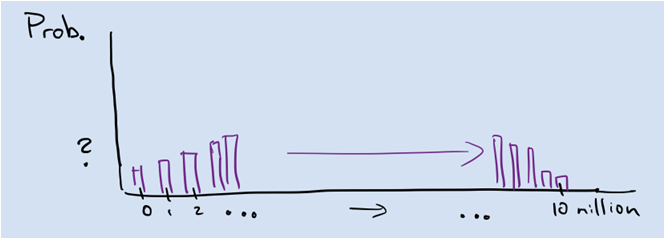
\includegraphics[scale=.5]{Bild16}
	           \end{figure}
	        \end{column}
	    \end{columns}
	\end{frame}
	
	
	
	\begin{frame}[c]{Abstracting Random Chance}
	    Q: What do these have in common?\\
	    \bigskip
	    \begin{columns}
	        \begin{column}{.3\textwidth}
	            Ask a randomly drawn American who they plan to vote for
	        \end{column}
	        
	        \begin{column}{.3\textwidth}
	          The outcome of a coin flip\\
	          \bigskip
	          A: Each have only two outcomes, one of which happens with a particular probability p

	        \end{column}
	        
	        \begin{column}{.3\textwidth}
	          The outcome of a COVID test for a randomly selected Californian

	        \end{column}
	    \end{columns}
	\end{frame}
	
	
	\begin{frame}[c]{Bernoulli Distribution}
	    \begin{columns}
	        \begin{column}{.3\textwidth}
	             A random variable that takes the value 1 with probability p and 0 otherwise.\\
	            \begin{figure}
	                \centering
	                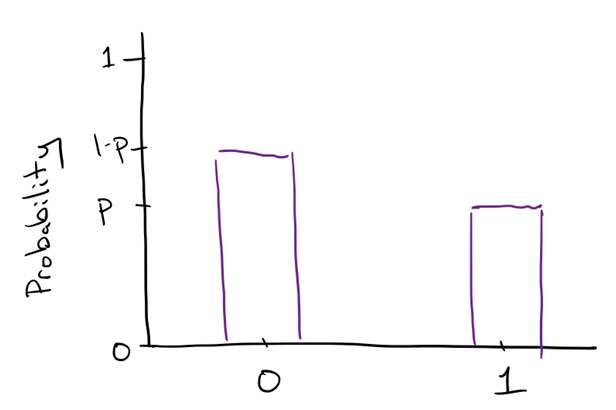
\includegraphics[scale=.6]{Bild17}
	            \end{figure}
	        \end{column}
	        
	        
	        \begin{column}{.5\textwidth}
	          X is Bernoulli(p) if:\\
	          \begin{itemize}
	              \item P(X = 1) = p
	              \item P(X = 0) = 1-p
	          \end{itemize}
              This is a Probability Mass Function (PMF)\\
              Examples:
              \begin{itemize}
                  \item Ask a randomly drawn American who they plan to vote for
                  \begin{itemize}
                      \item Bernoulli(p = .61)
                  \end{itemize}
                  \item The outcome of a coin flip
                  \begin{itemize}
                      \item Bernoulli(p = .5)
                  \end{itemize}
                  \item The outcome of a COVID test for a randomly selected Californian
                  \begin{itemize}
                      \item Bernoulli(p = .08)
                  \end{itemize}
              \end{itemize}
                
	        \end{column}
	    \end{columns}
	\end{frame}
	
	
	\begin{frame}[c]{Binomial Distribution}
	    \begin{columns}
	        \begin{column}{.4\textwidth}
	             A random variable that counts the number of “successes” in n independent trials where each succeeds with probability p.\\
	             \begin{figure}
	                 \centering
	                 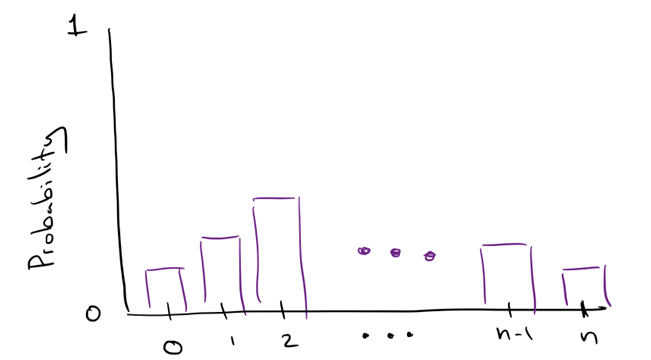
\includegraphics[scale=.5]{Bild19}
	             \end{figure}
	        \end{column}
	        
	        \begin{column}{.4\textwidth}
	         \begin{figure}
	             \centering
	             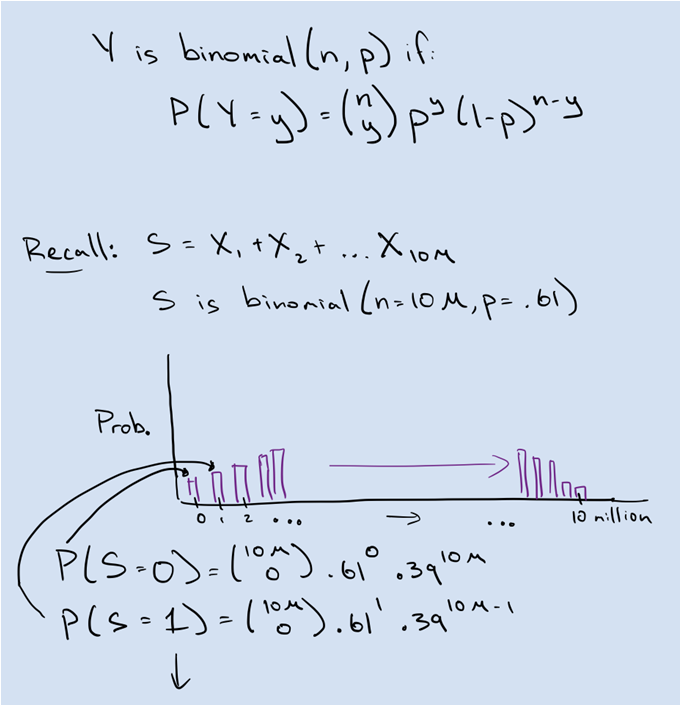
\includegraphics[scale=.5]{Bild18}
	         \end{figure}
	        \end{column}
	    \end{columns}
	\end{frame}
	
	
	\begin{frame}[c]{Abstracting Random Chance}
	    Q: What do these have in common?\\
	    \bigskip
	    \begin{columns}
	        \begin{column}{.3\textwidth}
	            Count the number of people that answered “FDR” in a sample of n = 10M\\
	            \bigskip
	            Binomial(n = 10M, p = .61)
	            \begin{itemize}
	                \item BUT each X$_i$ is not quite independent with the same p

	            \end{itemize}
	        \end{column}
	        
	        \begin{column}{.3\textwidth}
	          The total number of heads in a series of 5 coin flips\\
	          \bigskip
	          Binomial(n = 5, p = .5)
	          \begin{itemize}
	              \item Good fit!
	          \end{itemize}

	        \end{column}
	        
	        \begin{column}{.4\textwidth}
	          A random variable that counts the number of “successes” in n independent trials where each succeeds with probability p.\\
	          \bigskip
	          The total number of Californians that will test positive for COVID in a given month.\\
              \sout{Binomial(n = .5M, p = .08)}
              \begin{itemize}
                  \item \sout{probably not independent}
                  \begin{itemize}
                  \item \sout{contagious!}
                  \end{itemize}
                  \item \sout{probably not a good fit}
              \end{itemize}


	        \end{column}
	    \end{columns}
	\end{frame}
	
	
	\begin{frame}[c]{Types of distributions}
	    Probability distributions largely fall into two main categories.\\
	    \begin{itemize}
	        \item Discrete.
	        \begin{itemize}
	            \item The set of possible values that X can take on is either finite or countably infinite.
	            \item Values are separated by some fixed amount. 
	            \item For instance, X = 1, 2, 3, 4, …
	        \end{itemize}
	        \item Continuous.
	        \begin{itemize}
	            \item The set of possible values that X can take on is uncountable.
	            \item Typically, X can be any real number in some interval (not just our counting numbers).
	        \end{itemize}
	    \end{itemize}
	    Here, we will focus almost exclusively on discrete distributions. However, it’s important to know that continuous distributions exist. They will reappear later on! (bias-variance tradeoff, KDEs).

	\end{frame}
	
	
	\begin{frame}[c]{Common distributions}
	   \begin{columns}
	        \begin{column}{.4\textwidth}
	             Discrete
	             \begin{itemize}
	                 \item Bernoulli (p).
	                 \begin{itemize}
	                     \item Takes on the value 1 with probability p, and 0 with probability 1-p.
	                 \end{itemize}
	                 \item Binomial (n, p).
	                 \begin{itemize}
	                     \item Number of 1s in n independent Bernoulli (p) trials.
	                     \item Probabilities given by the binomial formula.
	                 \end{itemize}
	                 \item Uniform on a finite set.
	                 \begin{itemize}
	                     \item Probability of each value is 1 / (size of set). For example, a standard die.
	                 \end{itemize}
	             \end{itemize}
	        \end{column}
	        
	        \begin{column}{.4\textwidth}
	         Continuous
	         \begin{itemize}
	             \item Uniform on the unit interval.
	             \begin{itemize}
	                 \item U could be any real number in the range [0, 1]. 
	             \end{itemize}
	             \item Normal ($\mu,\sigma^2$)
	         \end{itemize}
	         Parameters of a distribution are the constants associated with it. These define its shape and the values it takes on. These are the numbers provided in parentheses. (\url{https://ismay.shinyapps.io/ProbApp/})


	        \end{column}
	    \end{columns}

	\end{frame}
	
	\begin{frame}[c]{Poll }
	   How many total heads would you expect to get in 5 flips of a fair coin?
	\end{frame}
	
	
	
	
	\begin{frame}[c]{Common distributions}
	       Expected Value\\
	            The expected value of a random variable X is the weighted average of the values of X, where the weights are the probabilities of the values.

	   \begin{columns}
	        \begin{column}{.4\textwidth}
	            \begin{figure}
	                \centering
	                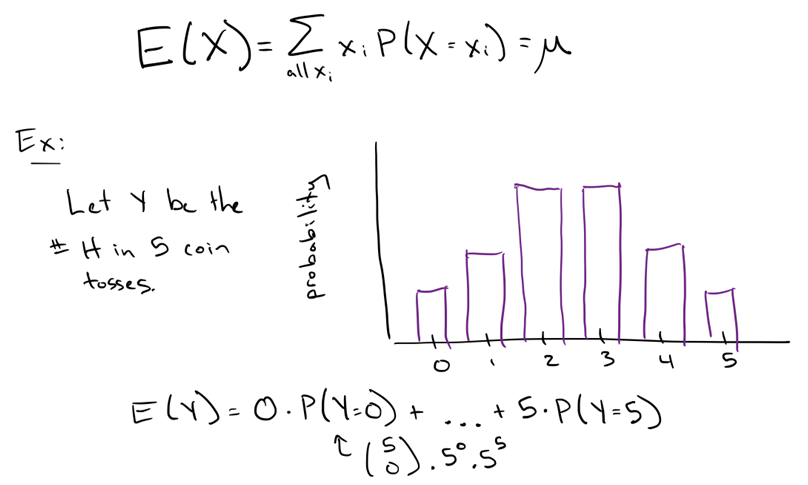
\includegraphics[scale=.5]{Bild20}
	            \end{figure}
	        \end{column}
	            
	        \begin{column}{.4\textwidth}
	            \begin{itemize}
	                \item Expected value is a number, not a random variable
	                \item It is analogous to the average.
	                \begin{itemize}
	                    \item It has the same units as the random variable
	                    \item It doesn’t need to be a possible value of the random variable.
	                    \item It is the center of gravity of the probability histogram.
	                \end{itemize}
	            \end{itemize}
	        \end{column}
	    \end{columns}

	\end{frame}
	
	
	\begin{frame}{Properties of Expectations}
	      Linear transformations\\
          Let Z = aX +b;\hspace{2cm} $\mathbb{E}(Z) = \mathbb{E}(aX + b) = a\mathbb{E}(X) + \mathbb{E}(b) = a\mathbb{E}(X) + b$ \\
          \bigskip
          Additivity\\
          Let W = $X_1 + X_2$;\hspace{2cm} $\mathbb{E}(W) = \mathbb{E}(X_1 + X_2) = \mathbb{E}(X_1) + \mathbb{E}(X_2)$ \\
          \bigskip
	      Linearity of Expectation\\
	      Let W = $aX_1 + bX_2$;\hspace{2cm} $\mathbb{E}(V) = \mathbb{E}(aX_1 + bX_2) = a\mathbb{E}(X_1) + b\mathbb{E}(X_2)$ \\
            
	  
	\end{frame}
	
	
	\begin{frame}[c]{Calculating Expected Values}
	   \begin{columns}
	        \begin{column}{.4\textwidth}
	        Bernoulli\\
	        Let X be Bernoulli(p)\\
	        \begin{align*}
	            \mathbb{E}(X) &= \sum\limits_k k\mathbb{P}(X=k)\\
	            &= 0(1-p)+1p\\
	            &= p
	        \end{align*}
	            \begin{figure}
	                \centering
	                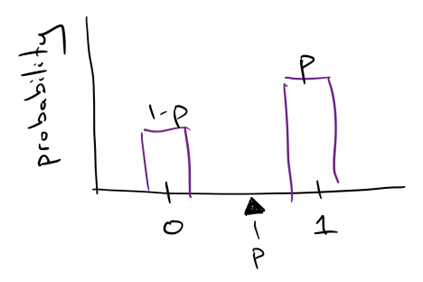
\includegraphics[scale=.5]{Bild21}
	            \end{figure}
	        \end{column}
	            
	        \begin{column}{.4\textwidth}
	            Binomial\\
	            Let Y be Binomial(n, p)\\
	            $Y=X_1+X_2+...+X_n$
	       \begin{align*}
	            \mathbb{E}(Y) &= \mathbb{E}(X_1) +\mathbb{E}(X_2) + ...+\mathbb{E}(X_n)\\
	            &= p + p +...+p\\
	            &= np
	        \end{align*}
	            \begin{figure}
	                \centering
	                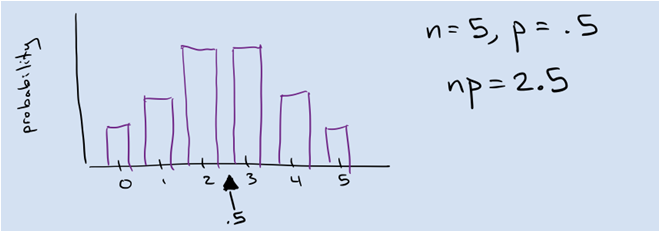
\includegraphics[scale=.5]{Bild22}
	            \end{figure}
	        \end{column}
	    \end{columns}

	\end{frame}
	
	
	
	
	\begin{frame}{Random Variables: Summary}
	      \begin{itemize}
	          \item In order to understand the world, you need to know how your data was generated
	          \item Random Variables and their distribution formalize that process
	          \item Many RVs reoccur and have been given names
	          \item One of the most prominent features of an RV is its expected value.
	      \end{itemize}
	  
	\end{frame}
	
\end{document}